\documentclass[a4paper, 12pt]{report}


%%%%%%%%%%%%%%%%%%
%   Liste des packages utilisés  %
%%%%%%%%%%%%%%%%%%

\usepackage{float}
\usepackage{lmodern} %Pack de police
\usepackage{graphicx}
\usepackage[utf8x]{inputenc}
\usepackage[T1]{fontenc}
\usepackage[francais]{babel}
\usepackage{caption}
\usepackage[top=2cm, bottom=2cm,left=2cm, right=2cm]{geometry}
\usepackage{setspace}
\usepackage{fancyhdr}
\usepackage{titlesec, blindtext, color} % titres spéciaux + couleur pour les chapter

% on transforme les chapters en juste le numéro suivi du titre, avec un barre grise
\definecolor{gray75}{gray}{0.75}
\newcommand{\hsp}{\hspace{20pt}}
\titleformat{\chapter}[hang]{\Huge\bfseries}{\thechapter\hsp\textcolor{gray75}{|}\hsp}{0pt}{\Huge\bfseries}


%Définition du style des bords de page
\pagestyle{fancy}
\renewcommand{\chaptermark}[1]{\markboth{\bsc{\thechapter{}- } #1}{}}
\lhead{}
\chead{}
\rhead{\leftmark}
\lfoot{Groupe n\up{o}2}
\cfoot{}
\rfoot{Page \thepage}

\fancypagestyle{plain}{%
    \lhead{}
    \chead{}
    \rhead{}
    \renewcommand{\headrulewidth}{0pt}
    \lfoot{Groupe n\up{o}2}
    \cfoot{}
    \rfoot{Page \thepage}
}

\begin{document}

%%%%%%%%%%%
%  Page de garde  %
%%%%%%%%%%%
\begin{titlepage}



	\begin{spacing}{1.5}
			\begin{minipage}{0.4\textwidth}
					
\includegraphics[width=3cm]{logo.png}
			\end{minipage}
			\begin{minipage}{0.5\textwidth}\raggedleft
					RuÞycross\\
			\end{minipage}
						\vspace*{\fill}

	\end{spacing}



	\begin{center}
		\begin{spacing}{2}
		    \hrule \vspace{1cm}
			\textbf{\huge Manuel Utilisateur}\\
			\vspace{1cm}
			\begin{minipage}{0.4\textwidth}
					\centerline{
\includegraphics[width=3cm]{test_logo_2.png}}
			\end{minipage}
			\vspace{1cm}
			\hrule

			\vspace*{\fill}


		\end{spacing}

		\begin{spacing}{1.15}
			\large\textbf{Groupe n\up{o}2} :\\
			\large
			\textsc{Brinon} Baptiste\\
			\textsc{Brocherieux} Thibault\\
			\textsc{Cohen} Mehdi\\
			\textsc{Debonne} Valentin\\
			\textsc{Lardy} Anthony\\
			\textsc{Mottier} Emeric\\
			\textsc{Pastouret} Gilles\\
			\textsc{Pelloin} Valentin\\
			\vspace*{\fill}
			%\textbf{Groupe n\up{o}2} \\
			\textnormal{\large Licence Informatique\\ Le Mans Université\\ \today}
		\end{spacing}
		
	\end{center}
\end{titlepage}

%%%%%%%%%%
%    Sommaire    %
%%%%%%%%%%
\renewcommand{\contentsname}{Sommaire}
\tableofcontents
\thispagestyle{empty}
\thispagestyle{plain}



\chapter{Pré-requis pour l'installation}
\thispagestyle{empty}
\thispagestyle{plain}
    
    Pour pouvoir exécuter correctement l'application, vous devez au préalable :
    \begin{itemize}
        \item Posséder un ordinateur sous MacOS ou Linux;
        \item Avoir installé une version de Ruby ultérieure à la 2.2.2;
        \item Avoir installé une version de la librairie Gtk ultérieure à la 3.22;
    \end{itemize}


\chapter{Règles du jeu}
\thispagestyle{empty}
\thispagestyle{plain}


		\section{Le but du jeu}

            Le but du Picross est de noircir les cases d'une grille de jeu, afin de faire apparaître une image, un dessin... Ceci à l'aide des indices se situant en marge de la grille.
            
%           \begin{minipage}{0.4\textwidth}
% 					\centerline{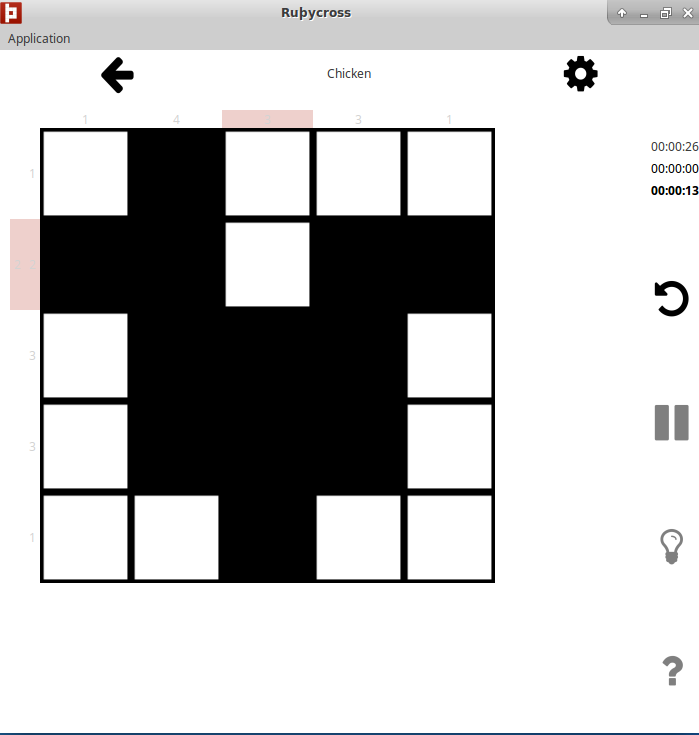
\includegraphics[width=3cm]{exempleGrille.png}}
% 			\end{minipage}

		\section{Les cases à noircir}
    
            Une grille comporte des indices en sa marge. Une ligne ou une colonne peut posséder un certain nombre d'indices :
            \begin{itemize}
                \item Les indices se situant à gauche de la grille permettant de connaître le nombre de cases à noircir sur la ligne correspondante.;
                \item Les indices se situant en haut de la grille permettent de connaître le nombre de cases à noircir sur la colonne correspondante.;
            \end{itemize}
	        
	        Ainsi, une grille possédant un nombre 5 devant une ligne ou une colonne indique qu'il y a 5 cases consécutives à noircir.
	        
	        Une grille possédant la séquence de nombre 2 3 devant une ligne ou une colonne indique qu'il y a un block de 2 cases à noircir, suivis d'au moins une case vide, puis un block de 3 cases à noircir.
	  
%           \begin{minipage}{0.4\textwidth}
% 					\centerline{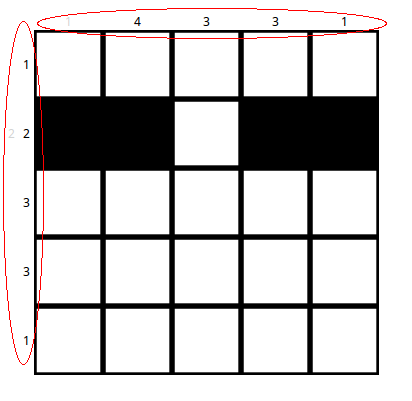
\includegraphics[width=3cm]{exempleIndice.png}}
% 			\end{minipage}
	       

		\section{Les cases faciles à noircir}

            Certaines astuces permettent de repérer les cases faciles à noircir, en voici quelques unes :
            \begin{itemize}
                \item Prenons par exemple un indice valant 10 sur une ligne d'une grille 10x10. Cela signifie que toutes les cases de la ligne en question sont à noircir.;
%           \begin{minipage}{0.4\textwidth}
% 					\centerline{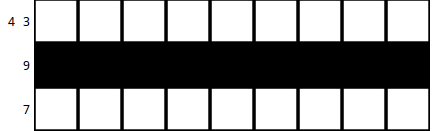
\includegraphics[width=3cm]{ligneExemple1.png}}
% 			\end{minipage}
                \item Prenons maintenant l'exemple d'une ligne ou une colonne dont l'indice est 3, et la première case est déjà noircie. Cela signifie que les cases à noircir sont obligatoirement les 3 premières.;
%           \begin{minipage}{0.4\textwidth}
% 					\centerline{\includegraphics[width=3cm]{ligneExemple2.png}}
% 			\end{minipage}
                \item Un dernier exemple : nous avons une grille 10x10, l'indice d'une des ligne vaut 7. On peut dans ce cas noircir les 4 cases centrales, ces cases seront noircies quelque soit la solution de cette ligne. Cette astuce fonctionne dès qu'une ligne ou une colonne possède un indice unique, supérieur à la moitié du nombre de cases de la ligne ou de la colonne en question.;
%           \begin{minipage}{0.4\textwidth}
% 					\centerline{\includegraphics[width=3cm]{ligneExemple3.png}}
% 			\end{minipage}
            \end{itemize}


		\section{Les cases à éliminer}
            
            Certaines cases sont à éliminer, elles ne sont donc pas à noircir, cela permet ainsi de voir plus clair dans la résolution d'une grille.
            
            Par exemple, les cases restantes d'une ligne contenant 5 cases à noircir, que vous avez déjà trouvées, sont à éliminer.

%           \begin{minipage}{0.4\textwidth}
% 					\centerline{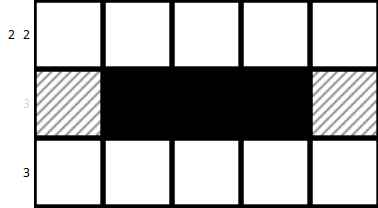
\includegraphics[width=3cm]{ligneExemple4.png}}
% 			\end{minipage}



\chapter{Guide pas à pas}
\thispagestyle{empty}
\thispagestyle{plain}

	\section{Connexion}

        Une fois l'application exécutée, vous avez la possibilité de sélectionner un compte, puis de cliquer sur le bouton "Connexion" afin d'accéder au menu du jeu. \\
        Pour ajouter un nouveau compte, vous devez cliquer sur le bouton "Créer un nouveau compte", et choisir votre pseudo.
        
        Sur cet écran, vous avez aussi la possibilité de changer la langue du jeu. Actuellement les langues disponibles sont :
        \begin{itemize}
            \item Le français,;
            \item L'anglais.;
        \end{itemize}
        
%           \begin{minipage}{0.4\textwidth}
% 					\centerline{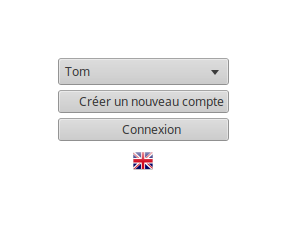
\includegraphics[width=3cm]{screenMenuCo.png}}
% 			\end{minipage}

	\section{Menu d'accueil}

	    Une fois connecté, vous avez accès au menu du jeu. Sur cet écran vous avez plusieurs possibilités :
	    \begin{itemize}
            \item Le bouton "Jouer" permet d'accèder au menu de choix de chapitres (cf : Jeu).;
            \item Le bouton "Classement" permet de visualiser vos statistiques de jeu.;
            \item Le bouton "Règles" permet de détailler les règles du jeu.;
            \item Le bouton "Options" donne la possibilité de changer :
            \begin{itemize}
                \item La langue (sont disponibles actuellement : le français et l'anglais),;
                \item La couleur des hypothèses (cf : [Insérez un numéro de chapitre]),;
                \item Les raccourcis clavier.;
            \end{itemize}
            Une fois vos changements effectués, pensez à appuyer sur le bouton "Valider".
            \item Le bouton "Quitter" permettant de fermer l'application.
        \end{itemize}

%           \begin{minipage}{0.4\textwidth}
% 					\centerline{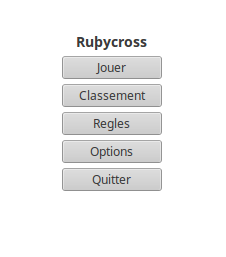
\includegraphics[width=3cm]{screenMenuJeu.png}}
% 			\end{minipage}


	\section{Jeu}

        \subsection{Choix des chapitres}
        
            Après avoir appuyé sur le bouton "Jouer", vous vous retrouvez sur le menu de choix de chapitre.
            Par défaut, seul le premier chapitre est disponible. Les suivants se débloquent au fur et à mesure de votre progression, en acquérant des étoiles. 
            Ces étoiles s'obtiennent en finissant des grilles d'un chapitre.
            
            Un chapitre est un regroupement thématique de plusieurs grilles. Ainsi le premier chapitre "Animaux" sera composé uniquement d'images liées aux animaux. 
            
%           \begin{minipage}{0.4\textwidth}
% 					\centerline{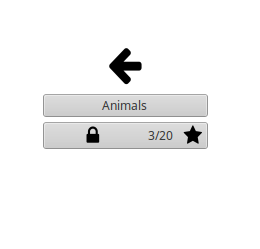
\includegraphics[width=3cm]{screenChoixChapitre.png}}
% 			\end{minipage}
            
        \subsection{Déroulement d'une partie} % à compléter
        
            Lorsque vous avez sélectionné la grille sur laquelle vous voulez jouer, une nouvelle interface apparaît. 
            Vous pouvez ainsi y retrouver :
            \begin{itemize}
                \item La grille de jeu.;
                Sur cette grille, vous pouvez colorier une case grâce à un clique gauche. Vous pouvez également sélectionner plusieurs cases d'un coup en maintenant le bouton gauche de la souris enfoncé.
                Le clique droit quant à lui permet de "cocher" une case que vous pensez fausse, afin de rendre la grille plus lisible. Le clique droit enfoncé permet également de sélectionner plusieurs cases.
                \item Trois timers : ;
                \begin{itemize}
                    \item Le premier étant le temps mis pour résoudre la grille en cours,;
                    \item Le deuxième, le temps de pénalité, lié aux aides, qui sera cumulé au temps total à la résolution de la grille,;
                    \item Le dernier, le temps estimé pour résoudre la grille.;
                Le nombre d'étoiles gagnées lors de la résolution totale d'une grille dépend du temps mis pour la résoudre.
                \end{itemize}
                \item Un bouton permettant de recommencer la grille;
                \item Un bouton de pause. Une fois le jeu mis en pause, le chronomètre est arrêté et la grille cachée. Vous pouvez à tout moment reprendre la partie, la grille réapparaîtra et le chronomètre se reprendra.;
                \item Les boutons d'aide ====>(à détailler)<====;
                \item Un bouton permettant d'accéder aux paramètres.;
            \end{itemize}
            
%           \begin{minipage}{0.4\textwidth}
% 					\centerline{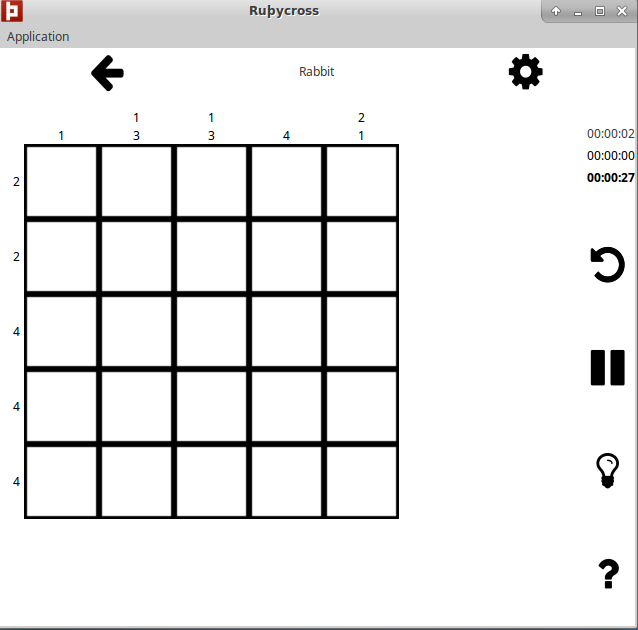
\includegraphics[width=3cm]{imageGrilleJeu.png}}
% 			\end{minipage}

        \subsection{Fin d'une partie}
        
            Une partie prend fin lorsque la grille est terminée et correcte. Une fenêtre s'ouvre alors en indiquant le temps mis pour résoudre la grille, ainsi que le nombre d'étoiles obtenues.
 
%           \begin{minipage}{0.4\textwidth}
% 					\centerline{\includegraphics[width=3cm]{imageGrilleFinJeu.png}}
% 			\end{minipage}          
            
	
	\section{Statistiques}

		

		
%	``I always thought something was fundamentally wrong with the universe'' \citep{adams1995hitchhiker}	
		\bibliographystyle{plain}
		\bibliography{references}

\end{document}
